\documentclass[a4paper 12pt]{article}

\usepackage{fullpage} % Package to use full page
\usepackage{parskip} % Package to tweak paragraph skipping
\usepackage{tikz} % Package for drawing
\usepackage{amsmath}
\usepackage{hyperref}

%\usepackage{sketch}
\begin{document}

\title{REPORT \#2 \\
   Numerical Methods in Solid and Fluid Mechanics}
\author{Claudio Pierard \\ Ekene Alexander Abanobi}
\date{21/12/2018}

\maketitle


%\chapter{INTRODUCTION}

\section{Aims and Objectives}
The objective of this practical work was modelling a distribution chain of a car under tension, and perform a static structural analysis in 3D. In particular, we wanted to calculate the maximum tensile stress applied to the chain considering a safety factor.

\section{Synthesis of the Study}

The chain distribution of a car consists of four types of pieces assembled together. In figure~\ref{fig:chain_scan} is possible to see the way in the four pieces are assembled to form the chain. In the figure, we can highlight that there are two types of links, an external one and an internal one.

%%%%%%%%%%%%%%%%% chain_scan %%%%%%%%%%%%%%%%%%%%%%%%%
\begin{figure}[!ht]
    \centering
    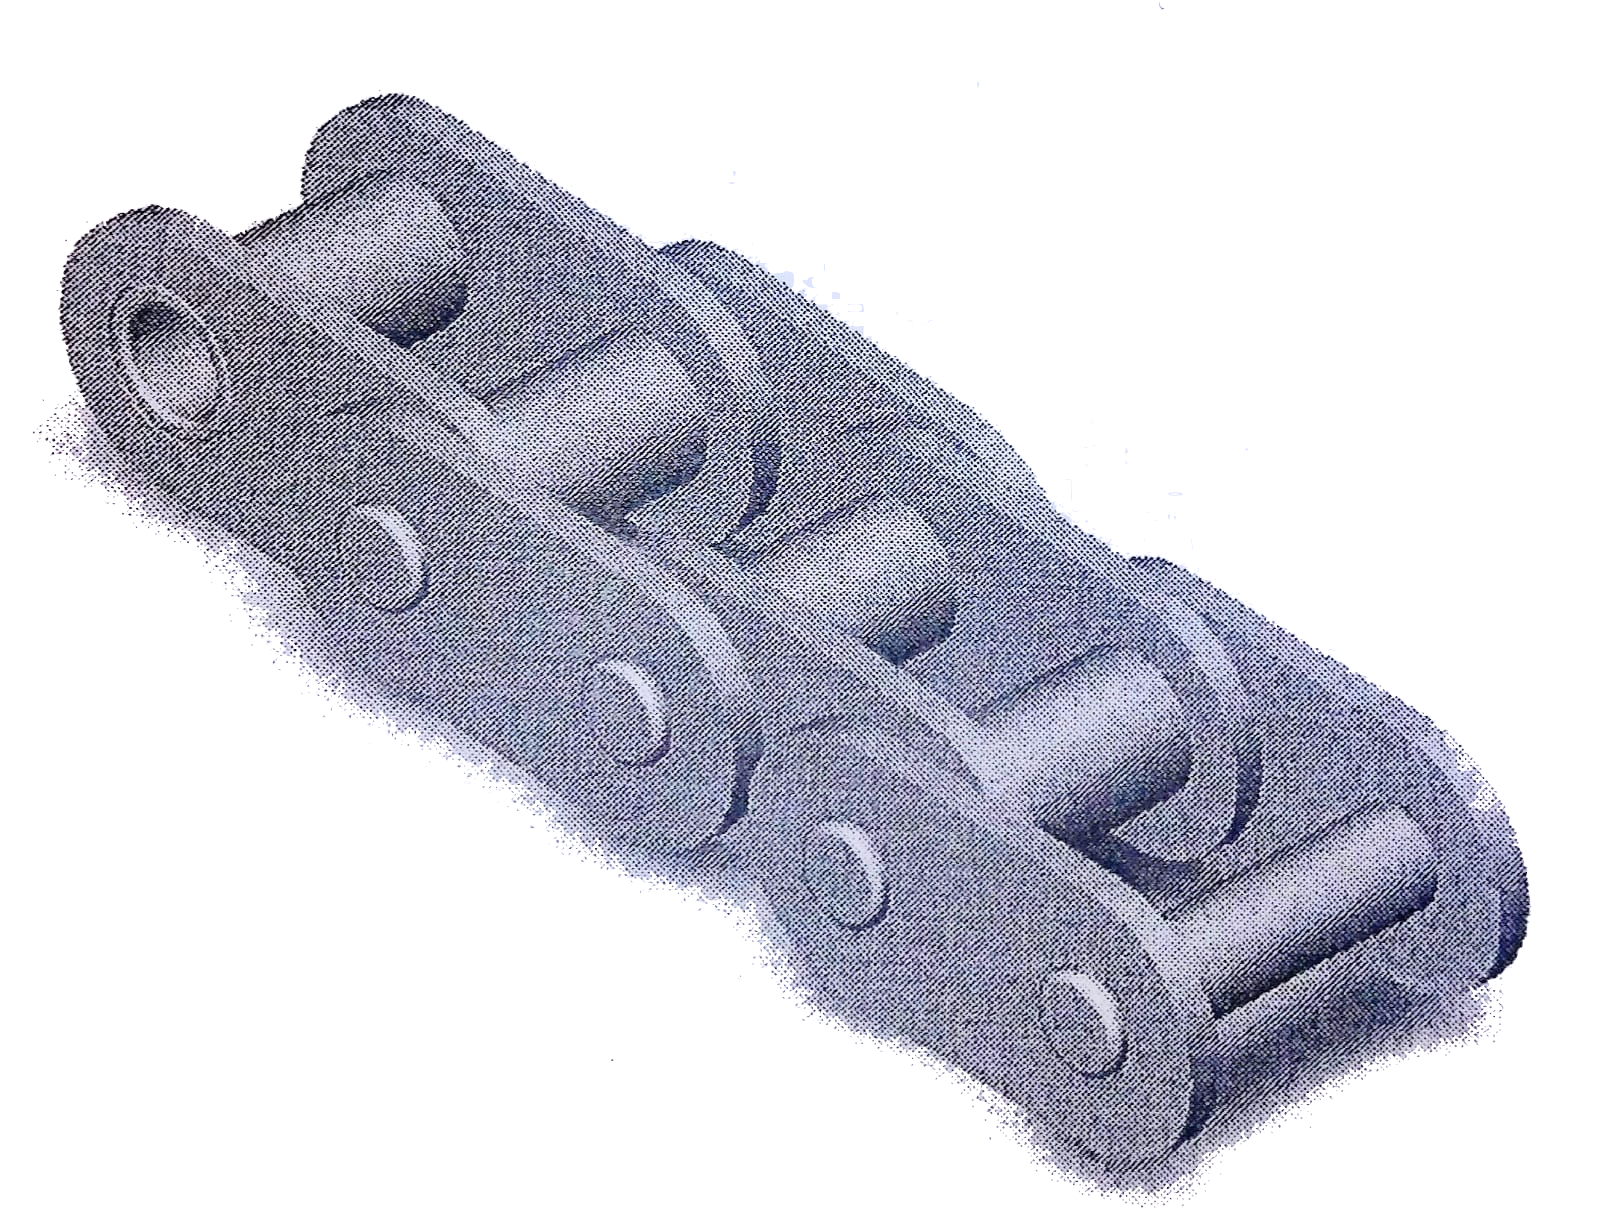
\includegraphics[width = 4cm]{images/chain_scan.png}
    \caption{Section of the distribution chain. It is possible to see the assembling of the pieces to form the chain.}
    \label{fig:chain_scan}
\end{figure}
%%%%%%%%%%%%%%%%%%%%%%%%%%%%%%%%%%%%%%%%%%%%%%%%%%%%%%%%%%%

The four pieces that make up the chain are shown in figure~\ref{chain_components}. From it, we distinguish two plates, one axis and one socket. In figure~\ref{fig:chain_scan} we can distinguish two types of plates in the chain. The plate A that is placed in the inner part of the chain, we call it inner plate, and the plate B placed in the outer part of the chain, we call it outer plate. Also, in figure~\ref{chain_components} we can see the axis, which correspond to the piece C, and the socket, which corresponds to the piece D.

The materials of the components of the chain are steel of different kinds depending on the part. For the plate, the material is steel XC55 with an elastic limit of 550~MPa. For the axis, the stell is XC65 with an elastic limit of 610~MPa. For the socket, the steel is 18CD4 with an elastic limit of 750~MPa.

%%%%%%% Chain links Sketch %%%%%%%%%
\begin{figure}[!ht]
\begin{center}
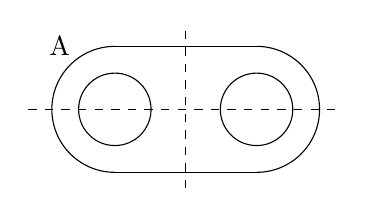
\begin{tikzpicture}[scale=0.2]
%\draw[red, thick, domain=0:2] plot(\x,0 * \x);
\draw [thin, -] (-4.5,4) -- (4.5,4);
\draw [thin, -] (-4.5,-4) -- (4.5,-4);
\draw (4.5,4) arc (90:-90:4);
\draw (-4.5,4) arc (90:270:4) (-8,4) node {A};
\draw(4.5,0) circle (2.3);
\draw(-4.5,0) circle (2.3);
\draw[thin,dashed] (-10,0) -- (10,0);
\draw[thin,dashed] (0,5) -- (0,-5);
\end{tikzpicture}
\qquad
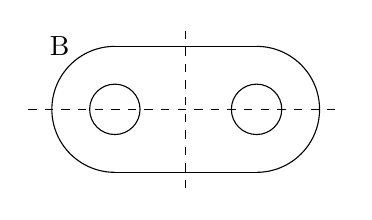
\begin{tikzpicture}[scale=0.2]
%\draw[red, thick, domain=0:2] plot(\x,0 * \x);
\draw [thin, -] (-4.5,4) -- (4.5,4) node [align=left, below]{};
\draw [thin, -] (-4.5,-4) -- (4.5,-4) node [align=left, below]{};
\draw (4.5,4) arc (90:-90:4);
\draw (-4.5,4) arc (90:270:4) (-8,4) node {B};
\draw(4.5,0) circle (1.6);
\draw(-4.5,0) circle (1.6);
\draw[thin,dashed] (-10,0) -- (10,0);
\draw[thin,dashed] (0,5) -- (0,-5);
\end{tikzpicture}
\qquad
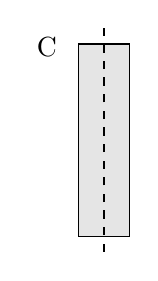
\begin{tikzpicture}[scale=0.2]
\filldraw[fill=gray!20](0,0) rectangle (3.25, 12.2);
\draw[thin,dashed] (1.625,-1) -- (1.625,13.2) (-2,12) node {C};
\end{tikzpicture}
\qquad
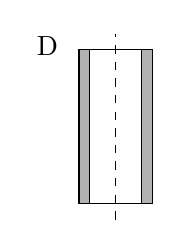
\begin{tikzpicture}[scale=0.2]
\filldraw[fill=gray!60] (0,0) rectangle (4.65,9.8) (-2,10) node {D};
\filldraw[fill=white!40] (0.675,0) rectangle (3.975,9.8);
\draw[thin,dashed] (2.325,-1) -- (2.325,10.8);
\end{tikzpicture}
\end{center}
\caption{The Four pieces that make up the chain. A is the inner plate, B is the outer plate, C is the axis and D is the socket.}
\label{chain_components}
\end{figure}
%%%%%%%%%%%%%%%%%%%%%%%%%%%%%%%%%%%%

The chain is under tension by means of pinions, which drive it at low speed to consider a static structural analysis. In other words, we assume that the chain is static and a force is applied in the direction along the chain moves.

%\chapter{METHODOLOGY}
\section{Methodology}

For modelling the chain we used ANSYS, which is software for 3D designing and performing simulations in a wide variety of problems. In this case, we used it to perform a static structural analysis of the chain. Maybe to do this we could have drawn all the components of the whole chain to model the entire chain, so the study would have been more realistic. The problem in doing this is that it would have taken us too much time, and the computational time for simulating the dynamics would have been very large. Instead of doing this, we reduced the problem to the fundamental pieces, taking into account that the same parts of the chain repeat them self many times. Also, we used the symmetries present in the chain to reduce the problem in the fundamental parts, and from them, infer the behaviour of the whole chain.

The first symmetry that we used to reduce the problem was the one that separates both sides of the chain in the direction were the chain moves. There are two sides that are symmetric that make up the chain, a pair of inner plates connected by the sockets and a pair of outer plates connected by the axis, and so on all along the chain. In this was, we are able to model just one side of the chain.

Figure~\ref{chain_union} is a sketch of the simplest connection of the chain that includes all the different parts. In this figure, we can see at the left the inner plate with the socket. Overlapped to the inner plate we see the outer plate with the axis. Also, we can see three dashed lines that cut through the chain. These lines are the axis of symmetry of the chain span and separate the chain span in 6 regions (labels 1 to 6). Parallel to the x-axis, we can see that there is an axis of symmetry in which the top part and the bottom part are similar. In other words, the regions 1, 2 and 3 are equivalent to the regions 4, 5, 6.

%%%%%%% Chain links Sketch %%%%%%%%%
\begin{figure}[!htbp]
\begin{center}
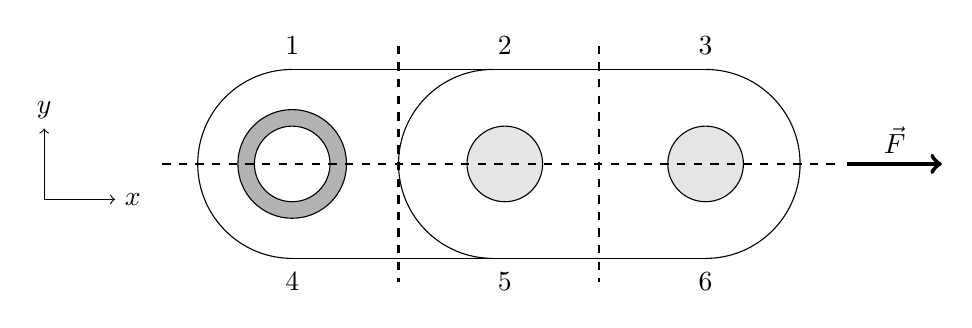
\begin{tikzpicture}[scale=0.3]
\draw [thin, -] (-4.5,4) -- (4.5,4);
\draw [thin, -] (-4.5,-4) -- (4.5,-4);
%\draw (4.5,4) arc (90:-90:4);
\draw (-4.5,4) arc (90:270:4);
\filldraw[fill=gray!20](4.5,0) circle (1.6) (-4.5,5) node {1};
\filldraw[fill=gray!60](-4.5,0) circle (2.3)(-4.5,-5) node {4};
\filldraw[fill=white!20](-4.5,0) circle (1.6)(4.5,5) node {2};
\draw [thin, -] (4,4) -- (13,4)(4.5,-5) node {5};
\draw [thin, -] (4,-4) -- (13,-4)(13,5) node {3};
\draw (13,4) arc (90:-90:4)(13,-5) node {6};
\draw (4,4) arc (90:270:4);
\filldraw[fill=gray!20](13,0) circle (1.6);
\draw[thick,dashed] (-10,0) -- (18.5,0);
\draw[thick,dashed] (0,5) -- (0,-5);
\draw[thick,dashed] (8.5,5) -- (8.5,-5) (21,1) node {$\Vec{F}$};
\draw[ultra thick, ->] (19,0) -- (23, 0);
\draw[->] (-15,-1.5) -- (-12,-1.5) node[right] {$x$};
\draw[->] (-15,-1.5) -- (-15,1.5) node[above] {$y$};
\end{tikzpicture}
\end{center}
\caption{Schematic of the section of consideration of the chain. The dashed lines are the axis of symmetry. From it, we can see that the section of consideration is divided into 6 sections (numbered in the top and bottom of sections). A force $\vec{F}$ is applied in the $x$-direction. The schematic is in the $y$-$x$ plane, with the $z$-axis coming outside of the page.}
\label{chain_union}
\end{figure}
%%%%%%%%%%%%%%%%%%%%%%%%%%%%%%%%%%%%

In figure~\ref{chain_union} as well, we can see two axes of symmetry parallel to the y-axis, in which the regions 1, 2 and 3 are similar (considering that there is an outer plate on region 1 and 4). This means that for studying the whole chain we can only simulate the region 2, in which the four different parts of the chain are involved. This implies that in the simulation we must only consider a quarter of each plate, and a semi-section of the axis and the socket. Also, is important to highlight that the force is applied in the positive x-direction.

Once we simplified as much as possible the problem, we proceeded to do the do the analysis of the reduced parts of the chain. The chain links are connected with the socket and the axis. The outer plate is fixed to the axis, and the inner plate is fixed to the socket. The axis goes inside of the socket and these two pieces are movable, which gives the chain its freedom of movement in the y-direction. In the static analysis is complex to perform the study of the four parts, including the movables parts. For this reason we decided to treat each piece separately and link each piece using the boundary conditions that correspond to each one of the pieces. Thereby, we explain separatly the condicion under which we made the analysis for each piece.

\subsection{Inner plate}

as already explained before, we took only a quarter of the plate because of the symmetries. We considered one of the superior querters. To perform the analysis we draw this piece in ANSYS workbench, and introduced the material properties like the elastic limit.

Following this, we stablished the boundary conditions for sufaces of the plate:

\begin{\begin{itemize}
  \item \textit{Bottom surface}: the surface is fix in the y-direction but is free to move in the x and z directions.
  \item \textit{Arc (surface inside the semicircle)}: In this surface we aplied the force in the positive x-direction.
  \item \textit{Lateral surfaces}: the lateral surfaces are free to move in the three directions.
  \item \textit{Side surce (symmetry with respect of the y-axis)}: this surface is set to move free in the y and z directions, but it cannot move in the x direction. This boundary condition opposes the force and with this we avoid the rigid body movement of the plate.
\end{itemize}}



Big plate:
Bottom surface: fix in the y component.
Lateral surface: fix in x direction
Inner surface of circle: force in x direction



\section{Link hypothesis}

Only the part of the axis in contact with the thickness of both plates was studied. This is so because the force we are studying is applied at two points (we more or less technically divided the axis into two). We studied the force applied at the surface of contact between the outer plate and the axis, also the force that is applied in between the surface of the inner plate and the axis. Another hypothesis is that under conditions of static equilibrium, these forces cancel out and are effectively equal and opposite and they create shear in the axis. Hence we considered only the outer part of the axis.

Bottom surface: Fixed in the y component:
This is so because the force is applied along the x-direction and hence x-direction cannot be constrained as it will cause an overconstrained system. It was also not constrained in the z-direction because that is the axis the deformation of will tend to (the z-axis) i.e. to give room for deformation.

Inner Lateral surface: This is fixed in the x and z directions
This surface is fixed in the x-direction even though the force is applied in the x-direction because we do not want rigid body motion (for the whole part under consideration to translate). It is also fixed in the z-direction because we are stating that the body under consideration is continuous in the z-direction i.e. taking into consideration that the axis has a length larger than the portion we are considering.


Outer Lateral Surface: This is FREE in all directions.
This is to make up for fixing the inner up for fixing the inner la


%\chapter{RESULTS}
\subsection{Outer Plate}

%%%%%%%%%%%%%%%%%%% Outer plate %%%%%%%%%%%%%%%%%%%%%%%%%
\begin{figure}[!ht]
    \centering
    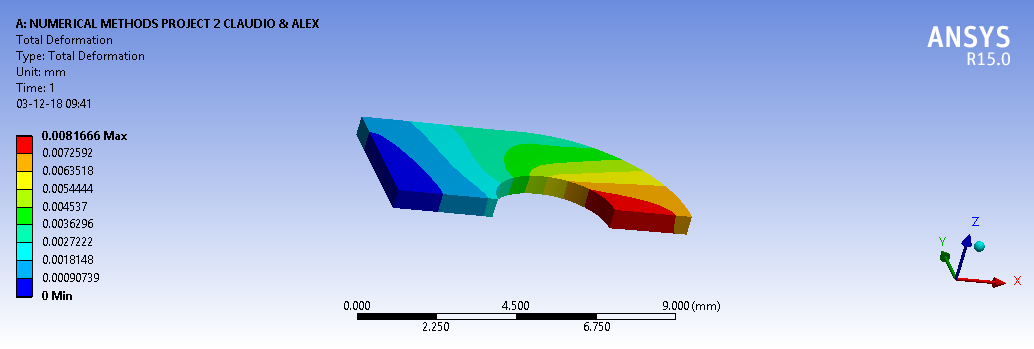
\includegraphics[width=1\textwidth]{images/OUTER_CHAIN_DEFORMATION.png}
    \caption{Caption}
    \label{fig:outer_deformation}
\end{figure}

\begin{figure}[!ht]
    \centering
    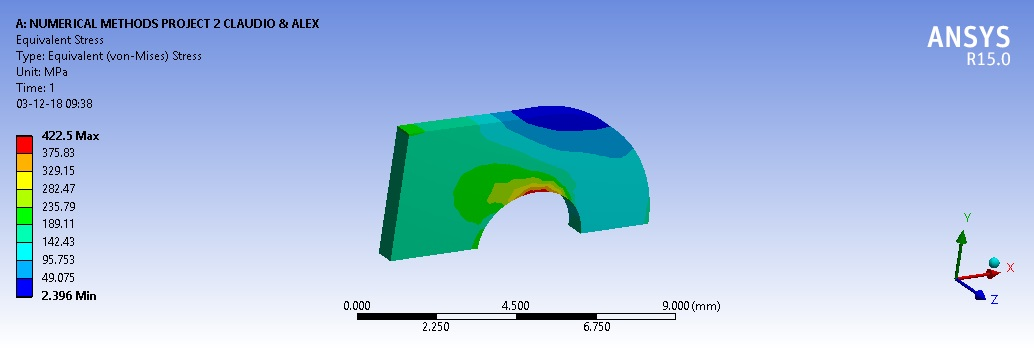
\includegraphics[width=1\textwidth]{images/CHAIN_SMALL_STRESS_TEST_FINAL.jpg}
    \caption{Caption}
    \label{fig:outer_stress}
\end{figure}
%%%%%%%%%%%%%%%%%%%%%%%%%%%%%%%%%%%%%%%%%%%%%%%%%%%%%%%%%%%


\subsection{Inner Plate}

%%%%%%%%%%%%%%%%%%%%%%% Inner plate %%%%%%%%%%%%%%%%%%%%%%%%
\begin{figure}[!ht]
    \centering
    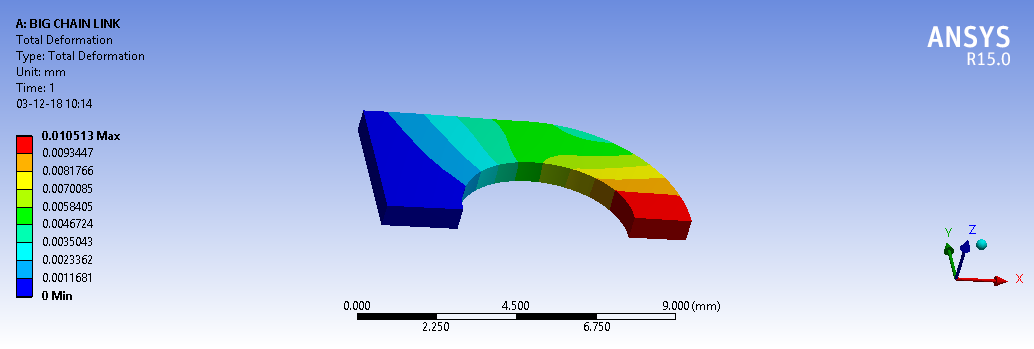
\includegraphics[width=1\textwidth]{images/INNER_CHAIN_DEFORMATION.png}
    \caption{Caption}
    \label{fig:inner_deformation}
\end{figure}

\begin{figure}[!ht]
    \centering
    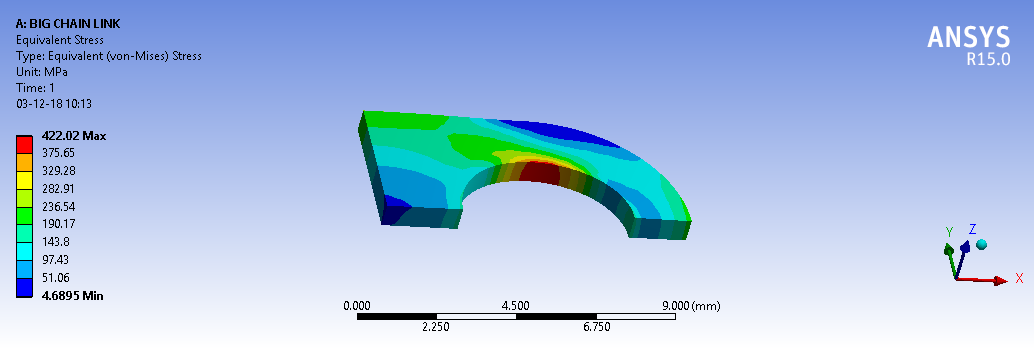
\includegraphics[width=1\textwidth]{images/INNER_CHAIN_STRESS.png}
    \caption{Caption}
    \label{fig:inner_stress}
\end{figure}
%%%%%%%%%%%%%%%%%%%%%%%%%%%%%%%%%%%%%%%%%%%%%%%%%%%%%%%%%%%

\subsection{Axis}

%%%%%%%%%%%%%%%%%%%%%%% Axis %%%%%%%%%%%%%%%%%%%%%%%%
\begin{figure}[!ht]
    \centering
    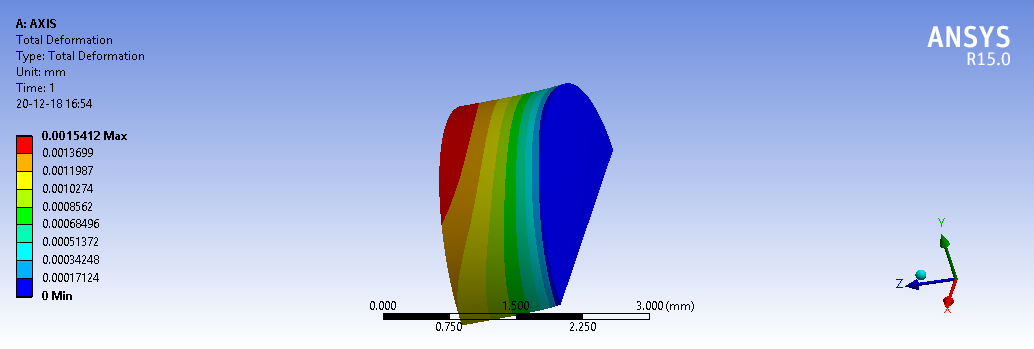
\includegraphics[width=1\textwidth]{images/AXIS_DISPLACEMENT.png}
    \caption{Caption}
    \label{fig:axis_deformation}
\end{figure}

\begin{figure}[!ht]
    \centering
    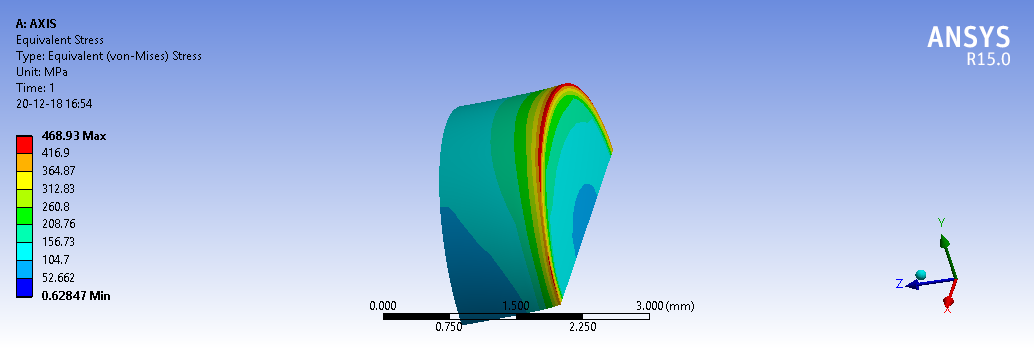
\includegraphics[width=1\textwidth]{images/AXIS_STRESS.png}
    \caption{Caption}
    \label{fig:axis_stress}
\end{figure}
%%%%%%%%%%%%%%%%%%%%%%%%%%%%%%%%%%%%%%%%%%%%%%%%%%%%%%%%%%%

\subsection{Socket}

%%%%%%%%%%%%%%%%%%%%%%% Socket %%%%%%%%%%%%%%%%%%%%%%%%
\begin{figure}[!ht]
    \centering
    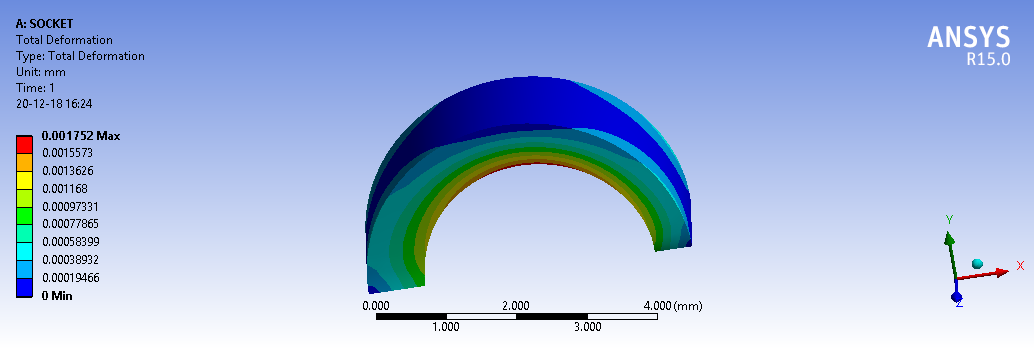
\includegraphics[width=1\textwidth]{images/SOCKET_DEFORMATION.png}
    \caption{Caption}
    \label{fig:socket_deformation}
\end{figure}

\begin{figure}[!ht]
    \centering
    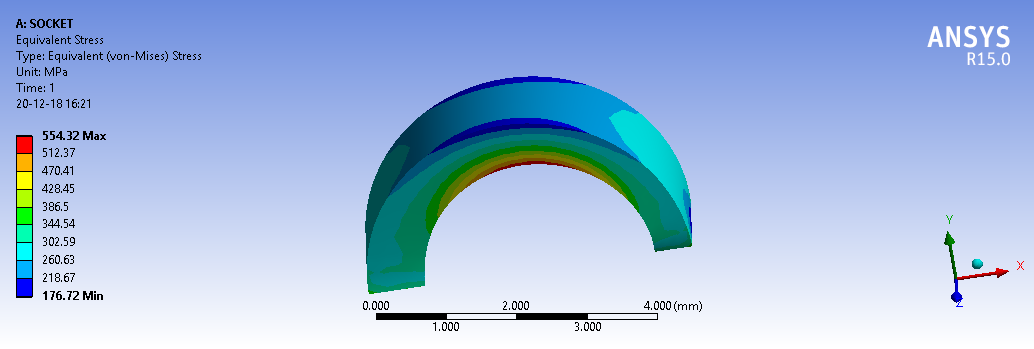
\includegraphics[width=1\textwidth]{images/SOCKET_STRESS.png}
    \caption{Caption}
    \label{fig:socket_stress}
\end{figure}
%%%%%%%%%%%%%%%%%%%%%%%%%%%%%%%%%%%%%%%%%%%%%%%%%%%%%%%%%%%


\begin{table}
\centering
\begin{tabular}{|p{4cm}|c|c|c|c|}
\hline
  & \textbf{Outer Plate (A)} & \textbf{Inner Plate (B)} & \textbf{Axis} & \textbf{Socket} \\
\hline
Theoretical Stress considering Elastic Limit [MPa] & 423 & 423 & 469 & 576 \\
\hline
Max. Force (Elastic Limit) [N] & 378 & 368 & 404.2 & 2500 \\
\hline
Equivalent Von-Mises Stress [MPa] & 422.5 & 422.02 & 468.93 & 554 \\
\hline
\end{tabular}
\caption{Comprehensive table of results}
\end{table}
%\chapter{CONCLUSION}

%\bibliographystyle{plain} %We don't have references, I think...
%\bibliography{bibliography.bib}
\end{document}
